%===============================================================================
\section{Revisión de Probabilidades}
%===============================================================================

%-----------------------------------------------------------------
\subsection{Elementos de probabilidad}
%-----------------------------------------------------------------
\begin{frame}{Espacio muestral}
	\begin{itemize}
		\item Aleatoriedada. Es la falta de (cierta) predictibilidad sobre situaciones.
		\item El resultado es un resultado potencial mutuamente excluyente de un proceso aleatorio.
		\item Un (sub) espacio muestral (S) es la unión de todas las posibles realizaciones o resultados.
		\item ¿Qué es un evento (A)?. Un evento es una realización o un subconjunto de realizaciones que pertenecen al espacio muestral (S).
		\item La probabilidad de ocurrencia es la proporción de eventos verificables que provienen de un proceso aleatorio.
		\item Axiomas de la probabilidad:
		\begin{itemize}
			\item \textit{Axioma 1}: $0\leq P(A) \leq 1$
			\item \textit{Axioma 2}: $P(S)=1$
			\item \textit{Axioma 3}: $P(UA_{i}) = \sum P(A_{i})$
		\end{itemize}
	\end{itemize}
\end{frame}
%------------------------------------------------
\begin{frame}{Algunos ejemplos}
	Indicar lso eventos de los siguientes (sub) espacios (S):
	{\small
		\begin{itemize}
			\item $A=$ \{x : x es el tipo de carros que se estrellaron en invierno\}
			\item $B=$ \{x : x es el número de computadoras destruidas cada 15 días\}
			\item $C=$ \{x : x es la nacionalidad de las personas en el salón de clases\}
			\item $D=$ \{x : x es el número de errores tipográficos en un documento cada 5 páginas\}
			\item $E=$ \{x : x es el tiempo de reacción de Usain Bolt en todas las carreras \}
			\item $F=$ \{x : x es el estudiante que falla en la pregunta número 1 del cuestionario\}
			\item $G=$ \{x : es una carta que pertenece a una baraja estandar\}
	\end{itemize}}
\end{frame}
%------------------------------------------------
\begin{frame}{Variable aleatoria}
	Las variables aleatorias (VA) son continuas o discretas. Una VA discreta solo toma un conjunto discreto de valores, mientras que una VA continua toma un posioble valor continuo. Por ejemplo:
	\begin{itemize}
		\item El número de personas que están en el salón depués de empezar cada clase.
		\item Puntaje en un cuestionario.
		\item Grados Fahrenheit o Celsius.
		\item Tiempo.
	\end{itemize}
	Puedes tranformar o convertir VA continuas en VA discretas fácilmente.
\end{frame}
%-----------------------------------------------------------------
\subsection{fdp y fda}
%-----------------------------------------------------------------
{\small
	\begin{frame}{Distribución probabilística y acumulada de una VA Discreta}
		La distribución de probabilidad es la probabilidad de que ocurra cada resultado o evento. Por ejemplo, observamos la cantidad de fallas de computadoras el primer día de clase; con base en una muestra de 10 estudiantes podemos construir la siguiente tabla:
		\begin{table}[!htbp]
			\centering
			\begin{tabular}{*7c}
				\hline
				{} &  \multicolumn{6}{c}{Resultados} \\
				{} & 0 & 1 & 2 & 3 & 4 & $\geq$5\\
				\hline
				Número  	 & 6 	& 0    & 3    & 0    & 1    & 0     \\
				fdp muestral & 0.60 & 0.00 & 0.30 & 0.00 & 0.10 & 0.000 \\
				fda muestral & 0.60 & 0.60 & 0.90 & 0.90 & 1.00 & 1.000 \\
				\hline
			\end{tabular}
		\end{table}
		formalmente, calculamos las probabilidades de la siguiente manera
		\begin{align*}
			&\textup{muestra base\, fdp}\enskip (\textup{fallas}=j) = \frac{(\#\textup{fallas}=j)}{n}\\
			&\textup{muestra base\, fda}\enskip (\textup{fallas}=j) = \sum_{i=0}^{j} 	\frac{(\#\textup{fallas}=j)}{n}
		\end{align*}
\end{frame}}
%------------------------------------------------
\begin{frame}{Histograma en diferentes tamaños de muestra}
	\begin{figure}
		\centering
		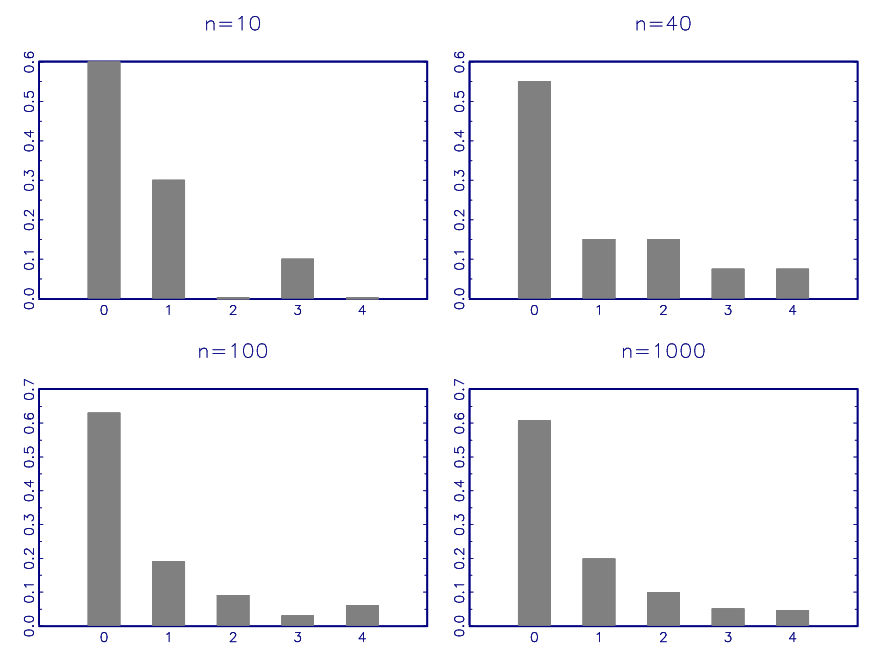
\includegraphics[scale=.40]{figuras/histograma_discr.png}
	\end{figure}
\end{frame}
%------------------------------------------------
{\small
	\begin{frame}{Distribución Bernoulli}
		Una distribución donde el resultado toma solo 2 valores: $0$ y $1$ es la distribución de Bernoulli. Es un caso particular de Distribución Binomial. Por ejemplo; Sea $G$ el género de la siguiente persona que ingrese al aula después de que comience la clase, donde $G=0$ indica que la persona es hombre y $G=1$ si esa persona es mujer. Los resultados de $G$ y sus probabilidades son:
		\begin{equation*}
			G =	\begin{cases}
				1\enskip \textup{con probabilidad}\enskip p\\
				0\enskip \textup{con probabilidad}\enskip 1-p
			\end{cases}
		\end{equation*}
		Además, podemos configurar un espacio con más de $2$ resultados pero finito. Por ejemplo, lanzar $2$ dados: $M$ es la suma de puntos en $2$ dados después de lanzarlos. Por lo tanto, $p(M=1)=0$
		\begin{gather*}
			p(M=2)= \frac{1}{36};p(M=3)= \frac{1}{36}; \ldots;p(M=7)= \frac{1}{36};\\
			\ldots \enskip \textup{y}\enskip p(M=12)= \frac{1}{36}
		\end{gather*}
\end{frame}}
%------------------------------------------------
\begin{frame}{Distribución probabilística y acumulada de una VA Continua}
	Por ejemplo, asumimos que las calificaciones se distribuyen normalmente con media y varianza iguales a 3 y 2 respectivamente.
	\begin{table}
		\centering
		\begin{tabular}{cccc}
			\hline
			Intervalo & Freq. Abs. & Freq. Rel. & Freq. Acum.\\
			\hline
			$[0;2[$  & 1.0 & 0.10 & 0.10\\
			$[2;4[$  & 4.0 & 0.40 & 0.50\\
			$[4;6[$  & 4.0 & 0.40 & 0.90\\
			$[6;8[$  & 1.0 & 0.10 & 1.00\\
			$[8;10]$ & 0.0 & 0.00 & 1.00\\
			\hline
		\end{tabular}
	\end{table}
\end{frame}
%------------------------------------------------
\begin{frame}{El histograma en diferentes tamaños de muestra.}
	\begin{figure}
		\centering
		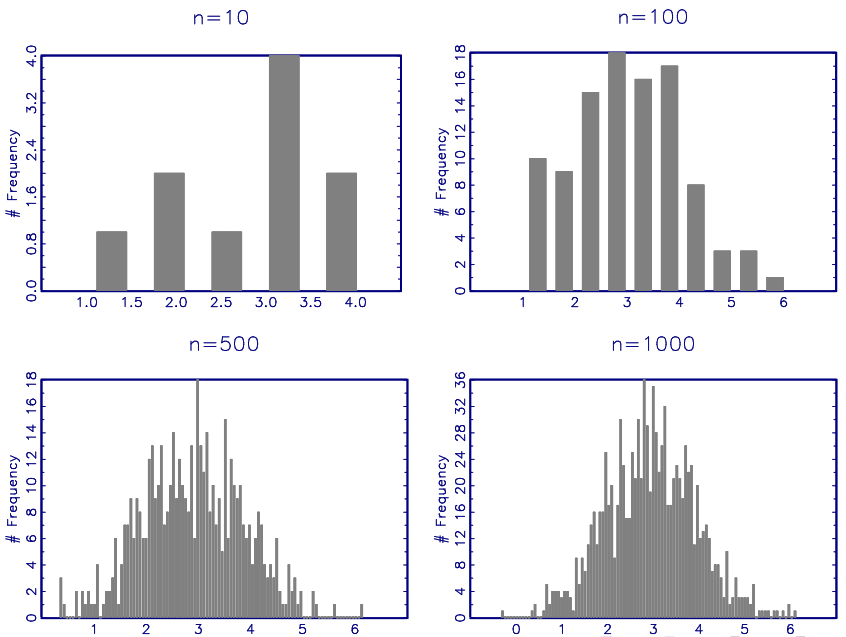
\includegraphics[scale=.40]{figuras/histograma_conti.png}
	\end{figure}
\end{frame}

%-----------------------------------------------------------------
\subsection{Valor esperado, media muestral y varianza}
%-----------------------------------------------------------------
\begin{frame}{Valor esperado, media muestral y varianza}
	Tenemos las siguientes definiciones y/o notaciones
	\begin{itemize}
		\item Variable aleatoria. Denotamos las variables aleatorias como $Y$.
		\item Una realización $i$ de $Y$. Es un resultado o valor observado. Denotamos eso como $y_{i}$.
		\item Valor esperado o media. Es el valor promedio a largo plazo de la variable aleatoria. Empíricamente, el valor esperado se puede aproximar como la media de la muestra cuando el número de observaciones o el tamaño de la muestra llega al infinito (o alcanza un número grande). Denotamos el valor esperado de una variable aleatoria como $E(Y)$ o $\mu_{Y}$.
		\item Media o promedio muestral. Es el valor promedio de la variable aleatoria. Denotamos la media de una variable aleatoria como $\mu_{Y, N}$.
		\item Diferencia. Es una medida de dispersión de la variable aleatoria. Denotamos la varianza como $\sigma_{Y}^{2}$.
	\end{itemize}
\end{frame}
%------------------------------------------------
\begin{frame}{Valor esperado, media muestral y varianza}
	Tome en cuenta que
	\begin{itemize}
		\item El valor esperada ($E$)  es un operador lineal.
		$$Eg(X) \geq g(E(X))$$
		\item Algunas reglas con constantes y variables aleatorias
		$$E(a+b) = a+b$$
		$$E(aX+b)=aE(X)+b$$
		$$E(XY)=E(X)E(Y) \textup{ si ambas variables son independientes}$$
	\end{itemize}
\end{frame}
%------------------------------------------------
\begin{frame}{Valor esperado (media), media muestral y varianza}
	Supongamos que tenemos las realizaciones para la variable $Y$. Por lo tanto,  tenemos $y_{1},\ y_{2},\ y_{3}, \ldots y_{k}$. También, conocemos las pobabilidad asociadas; estas son $p_{1},\ p_{2},\ p_{3}, \ldots 1 - \sum_{i}^{k-1}p_{y}$. Entonces, el valor esperado de $Y$, denotado por $E(Y)$ es $$E(Y) = p_{y_{1}}y_{1}+p_{y_{2}}y_{2}+p_{y_{3}}y_{3}+\ldots+p_{y_{k}}y_{k} = \sum_{i=1}^{k}p_{y_{i}}y_{i}$$ La suma anterior cubre todo el espacio de Y. En el caso de variables aleatorias continuas $$E(Y) = \int \limits_{\underline{y}}^{\bar{y}}yf(y)dy$$
\end{frame}
%------------------------------------------------
\begin{frame}{Desviación estandar y Varianza}
	La varianza de la variable aleatoria discreta $Y$ es $$\sigma_{Y}^{2} \equiv var(Y) = E[Y-\mu_{Y}]^2 = \sum_{i=1}^{k}(y_{i}-\mu_{k})^2p_{i}$$ En el caso de variables aleatorias continuas, la varianza es $$\sigma_{Y}^{2} \equiv var(Y) = E[Y-\mu_{Y}]^2 = \int \limits_{\underline{y}}^{\bar{y}}yf(y)dy$$ La desviación estandar de $Y$ es $\sigma_{Y}$ y es la raiz cuadrada de la varianza. ¿Cuál es la covarianza de las variables discretas y continuas?
\end{frame}
%------------------------------------------------
\begin{frame}{Ejercicio}
	Por ejemplo
	\begin{itemize}
		\item $G \thicksim B(1,p) \equiv B(p)$, entonces la media es $$E(G) = 0 \cdot  P(G=0) + 1 \cdot P(G=1)=p$$ y la varianza
		\begin{align*}
			\textup{var}(G) & \equiv E(G^2)-\mu_{G}^{2}\\
			& = 0^2 \cdot P(G=0)+1^2\cdot P(G=1)-p^2\\
			& = p(1-p)
		\end{align*}
		\item $X=5+G$, donde $G \thicksim B(p)$; entonces\\
		$E(X)=5\cdot P(G=0)+6P\cdot P(G=1)=5+p$;\\
		var$(X)= p(1-p)$
	\end{itemize}
\end{frame}
%------------------------------------------------
\begin{frame}
	\begin{itemize}
		\item $Y \thicksim N(0,1)$, entonces la media es $$E(Y)=0$$ y la varianza
		\begin{align*}
			\textup{var}(Y) & \equiv E(Y^2) - \mu_{Y}^{2}\\
			& = 1 
		\end{align*}
		\item $Z \thicksim N(5,2)$; entonces $E(Z)=5$; var$(Z)=2$
		\item $\frac{Z-5}{\sqrt{2}}\thicksim N(0,1)$
	\end{itemize}
\end{frame}
%------------------------------------------------
\begin{frame}{otros momentos}
	La curtosis es un indicador de cuánta masa hay en las colas de la distribución. El punto de referencia para este indicador es la distribución normal; en este caso la curtosis es igual a 3. La curtosis se calcula de la siguiente manera:
	$$\textup{Kurtosis} = E\left( \frac{Y-E(Y)}{\sigma_{Y}}\right)^4$$
	La asimetría es un indicador de la simetría de la distribución. Un valor positivo (negativo) indica que la distribución tiene una cola larga a la derecha (izquierda). El punto de referencia para este indicador es la distribución normal; en este caso, la asimetría es igual a 0. La asimetría se calcula de la siguiente manera
	$$\textup{Skewness} = E\left( \frac{Y-E(Y)}{\sigma_{Y}}\right)^3$$
\end{frame}
%------------------------------------------------
\begin{frame}{Una advertencia importante: valores esperados versus media muestral}
	Intente el siguiente ejercicio; descargue este conjunto de datos aquí. Luego, calcule las estadísticas de media, error estándar y covarianza para las ... primeras 5, 10, 50, 100 y 500 observaciones de la variable llamada rer y complete la siguiente tabla:\\
	\bigskip
	{\small
		\centering
		Estadísticas de muestra\\
		\smallskip
		\begin{tabular}{ cccc } 
			\hline
			Tamaño de muestra & Promedio & Error estandar & Cov con inf \\
			\hline
			5   & & & \\
			10  & & & \\
			50  & & & \\
			100 & & & \\
			50  & & & \\
			\hline
			\\                                                                                                                   
		\end{tabular}\\}
	Tener en cuenta que $E(rer) = 3$; var(rer)=2 y\\
	cov(rer,inf)=0.34
\end{frame}
%------------------------------------------------
\begin{frame}{Expresiones claves}
	Parámetros; $a, b, c \ldots;$ variables aleatorias $X, Y$
		\begin{align*}
			E(a+bX+cY) &=a+bE(X)+cE(Y)\\
			&=a+b\mu_{X}+c\mu_{Y}
		\end{align*}
		\begin{align*}
			Var(a+bX+cY) &=a^2Var(X)+b^2Var(Y)+2abCov(X,Y)\\
			&=a^2\sigma_{X}^{2}+b^2\sigma_{Y}^{2}+2ab\sigma_{XY}
		\end{align*}
		\begin{align*}
			Var(Y) & \equiv \sigma_{Y}^{2} = E(Y-E(Y))^2\\
			& = E(Y^2)-2E(Y)E(Y)+[E(Y)]^2\\
			& = E(Y^2) - [E(Y)]^2\\
			& = E(Y^2) - \mu_{Y}^{2}
		\end{align*}
\end{frame}
%------------------------------------------------
\begin{frame}{Expresiones claves}
	Parámetros; $a, b, c \ldots;$ variables aleatorias $X, Y$
		\begin{align*}
			\textup{cov}(X,Y) & \equiv E([X-E(X)][Y-E(Y)])\\
			& E(XY - E(X)Y-XE(Y)+E(X)E(Y))\\
			& E(XY-\mu_{x}Y-X\mu_{Y}+\mu_{X}\mu_{Y})\\
			& E(XY)-2\mu_{X}\mu_{Y}+\mu_{X}\mu_{Y}\\
			& E(XY)-\mu_{X}\mu_{Y}\\
			& \sigma_{XY}
		\end{align*}
	aquí $E(XY)$ se denomina covarianza bruta o no centrada entre $X$ e $Y$
\end{frame}

%-----------------------------------------------------------------
\subsection{Distribuciones conjuntas, marginales y condicionales}
%-----------------------------------------------------------------
\begin{frame}{Distribución conjunta}
	La distribución conjunta involucra al menos 2 variables aleatorias y es la probabilidad de observar resultados (asociados a estas variables aleatorias) simultáneamente.\\
	\smallskip
	{\small
		\centering
		Distribución conjunta\\
		\textcolor{red}{(en rojo)}\\
		\smallskip
		\begin{tabular}{c|cccc|c} 
			& \multicolumn{4}{c|}{Y} & \\
			X & 2 & 3 & 4 & 5 & Total \\
			\hline
			0 & \textcolor{red}{0.0} & \textcolor{red}{0.0}& \textcolor{red}{0.08} & \textcolor{red}{0.40} & 0.48 \\
			1 & \textcolor{red}{0.2}& \textcolor{red}{0.2}& \textcolor{red}{0.10} & \textcolor{red}{0.02} & 0.52 \\
			\hline
			Total & 0.2 & 0.2 & 0.18 & 0.42 & 1.00
		\end{tabular}\\}
	\medskip
	Según esta distribución la probabilidad de observar 5 fiestas asistidas y aprobar el curso de econometría $P (y = 5, x = 1)$ es del 2\%. Todos estos 8 eventos posibles son mutuamente excluyentes y constituyen el espacio muestral; las 8 probabilidades suman 1.
\end{frame}
%------------------------------------------------
\begin{frame}{Distribución marginal}
	La distribución marginal de una variable aleatoria es la distribución de probabilidad en sí. Esa es la probabilidad de observar resultados (asociada a esta variable aleatoria).\\
	\smallskip
	{\small
		\centering
		Distribución marginal\\
		\textcolor{blue}{(en azul)}\\
		\smallskip
		\begin{tabular}{c|cccc|c} 
			& \multicolumn{4}{c|}{Y} & \\
			X & 2 & 3 & 4 & 5 & Total \\
			\hline
			0 & 0.0 & 0.0& 0.08 & 0.40 & \textcolor{blue}{0.48} \\
			1 & 0.2& 0.2& 0.10 & 0.02 & \textcolor{blue}{0.52} \\
			\hline
			Total & \textcolor{blue}{0.2}& \textcolor{blue}{0.2}& \textcolor{blue}{0.18} & \textcolor{blue}{0.42} & 1.00
		\end{tabular}\\}
	\medskip
	Según esta distribución, la probabilidad de observar 5 fiestas $P (y = 5)$ es del 42\%. Los 4 posibles resultados de $Y$ son mutuamente excluyentes y constituyen un espacio muestral para $Y$; las 4 probabilidades suman 1.
\end{frame}
%------------------------------------------------
{\small
	\begin{frame}{Distribución condicional}
		La distribución condicional de una variable aleatoria es la distribución de probabilidad dada la realización de otra variable aleatoria. Formalmente, es la probabilidad de algún evento cuando el espacio muestral está restringido a otro evento.\\
		\smallskip
		{\centering
			Distribución condicional\\
			\textcolor{purple}{(en rojo)}\\
			\smallskip
			\begin{tabular}{c|cccc|c} 
				& \multicolumn{4}{c|}{Y} & \\
				X & 2 & 3 & 4 & 5 & Total \\
				\hline
				0 & \textcolor{purple}{0.0/0.2} & \textcolor{purple}{0.0/0.2}& \textcolor{purple}{0.08/0.18} & \textcolor{purple}{0.40/0.42} & n.d \\
				1 & \textcolor{purple}{0.2/0.2}& \textcolor{purple}{0.2/0.2}& \textcolor{purple}{0.10/0.18} & \textcolor{purple}{0.02/0.42} & n.d \\
				\hline
				Total & 1 & 1 & 1 & 1 & n.d
			\end{tabular}\\}
		
		\medskip
		Según esta distribución, la probabilidad condicional de observar un éxito en el curso (es decir, pasar la maldición) dado que asistieron 5 fiestas $P (x = 1 | y = 5)$ es 4.7\%. Todos los pares de probabilidades dados Y son mutuamente excluyentes y constituyen el espacio muestral dado un valor particular para Y; las 2 probabilidades suman 1 en cada caso.
\end{frame}}
%------------------------------------------------
\begin{frame}{Ejercicio}
	Calculemos la probabilidad marginal y condicional (dad la información de probabilidad conjunta) mediantes las siquientes expresiones
	$$P(Y=y) = \sum_{i=1}^{k}P(X=x, Y=Y) \quad (\textup{Pro. Marginal})$$
	$$P(Y=y|X=x) = \frac{P(X=x,Y=y)}{P(X=x)} \quad (\textup{Pro. Condicional})$$
	La última expresión es una aplicación del teorema de Bayes (es decir,$ P (A, B) = P (A | B) P (B)$)
\end{frame}
%------------------------------------------------
\begin{frame}{Expresiones claves adicionales}
	\begin{itemize}
		\item Esperanza condicional
		\begin{align*}
			E(Y|X=x) &= \sum_{i=1}^{I} y_{i} P(Y=y_{i}|X=x)\\
			&= \sum_{i=1}^{I}y_{i}\frac{P(X=x,Y=y_{i})}{P(X=x)}
		\end{align*}
		\item La ley de las expectativas iteradas (LEI)
		\begin{align*}
			E(Y) &= \underset{X}{E}[E(Y|X)]\\
			&= \sum_{i=1}^{k}E(Y|X=x_{i})P(X=x_{i})
		\end{align*}
	\end{itemize}
\end{frame}
%------------------------------------------------
\begin{frame}{Expresiones claves adicionales}
	\begin{itemize}
		\item Varianza condicional
			\begin{align*}
				\textup{var}(Y|X=x) = \sum_{i=1}^{I}[y_{i}-E(Y|X=x)]^2P(Y=y_{i}|X=x)
			\end{align*}
		\item Independencia
			\begin{align*}
				P(Y=y,X=x)=P(Y=y)P(X=x)
			\end{align*}
		\item Covarianza
			\begin{align*}
				\textup{cov}(Y,X)=\sum_{j=1}^{k}\sum_{i=1}^{I}[y_i-\mu_{Y}][x_j-\mu_{X}]P(Y=y_i,X=x_j)
			\end{align*}
	\end{itemize}
\end{frame}
%------------------------------------------------
\begin{frame}{Expresiones claves adicionales}
	\begin{itemize}
		\item Correlación (Parámetro de Pearson)
		$$\textup{corr}(X,Y)=\frac{\textup{cov}(X,Y)}{\sqrt{\textup{var}(Y)\textup{var}(X)}}$$
		La correlación mide la asociación estadística entre 2 variables (aleatorias). Se dice que las variables aleatorias no están correlacionadas si $\textup{corr}(X,Y)=0$. Es important mencionar que la correlación siempre está entre -1 y 1.
	\end{itemize} Además, debe tener en cuenta lo siguiente
	\begin{itemize}
		\item Si $E(Y|X) = \mu_{Y}$ (Independencia); entonces $\textup{cov}(X,Y)=0 \rightarrow \textup{corr}(X,Y) = 0$. La independencia no implica correlación, pero lo contrario no se cumple.
		\item $|\sigma_{X,Y}| \leq \sqrt{\sigma_{X}^{2}}\sqrt{\sigma_{Y}^{2}}$
		\item cov$(a+bX+cV,Y) = b\sigma_{X,Y} + c\sigma_{V,Y}$
	\end{itemize}
\end{frame}
%-----------------------------------------------------------------
\subsection{Distribuciones}
\begin{frame}{Distribución normal}
	El siguiente panel de gráficos muestra el fdp y el fda normal estándar.
		\begin{figure}
			\centering
			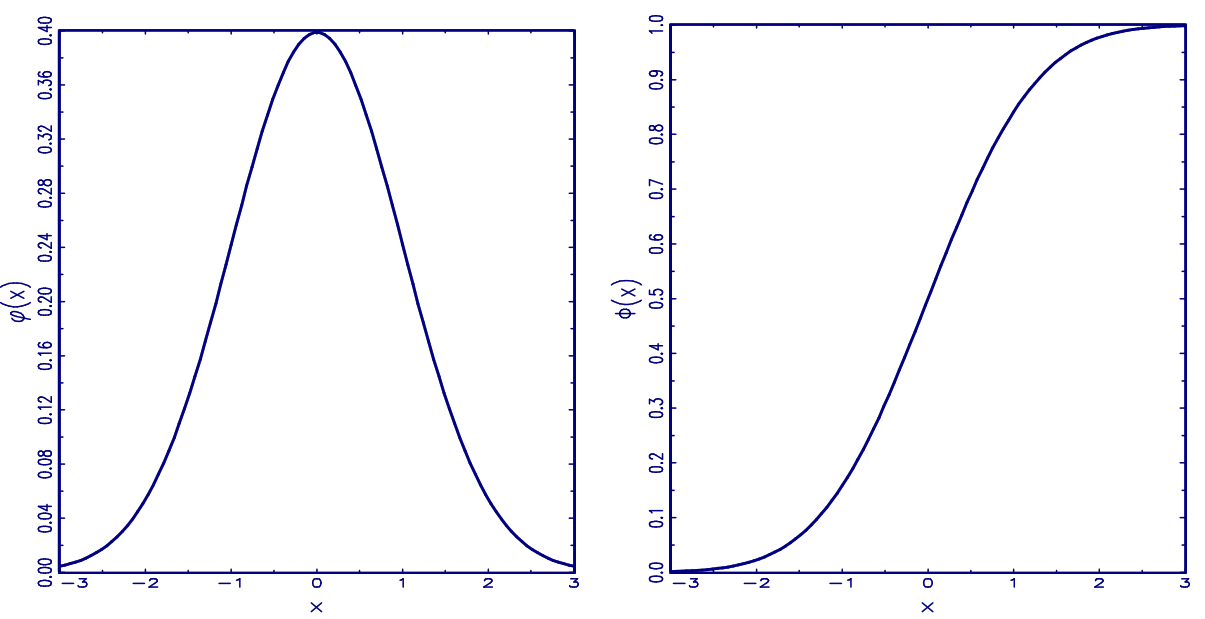
\includegraphics[scale=.22]{figuras/dist1.png}
		\end{figure}
	La distribución normal estandar se denota por $N(0,1)$.\\
	La fdp y fda se notan como $\phi(X)$ y $\Phi(X)$ respectivamente.
\end{frame}
%------------------------------------------------
\begin{frame}{Distribución Chi-Cuadrado}
	El siguiente panel de gráficos muestra la fdp y la fda de una Chi-cuadrado bajo diferentes grados de libertad.
		\begin{figure}
			\centering
			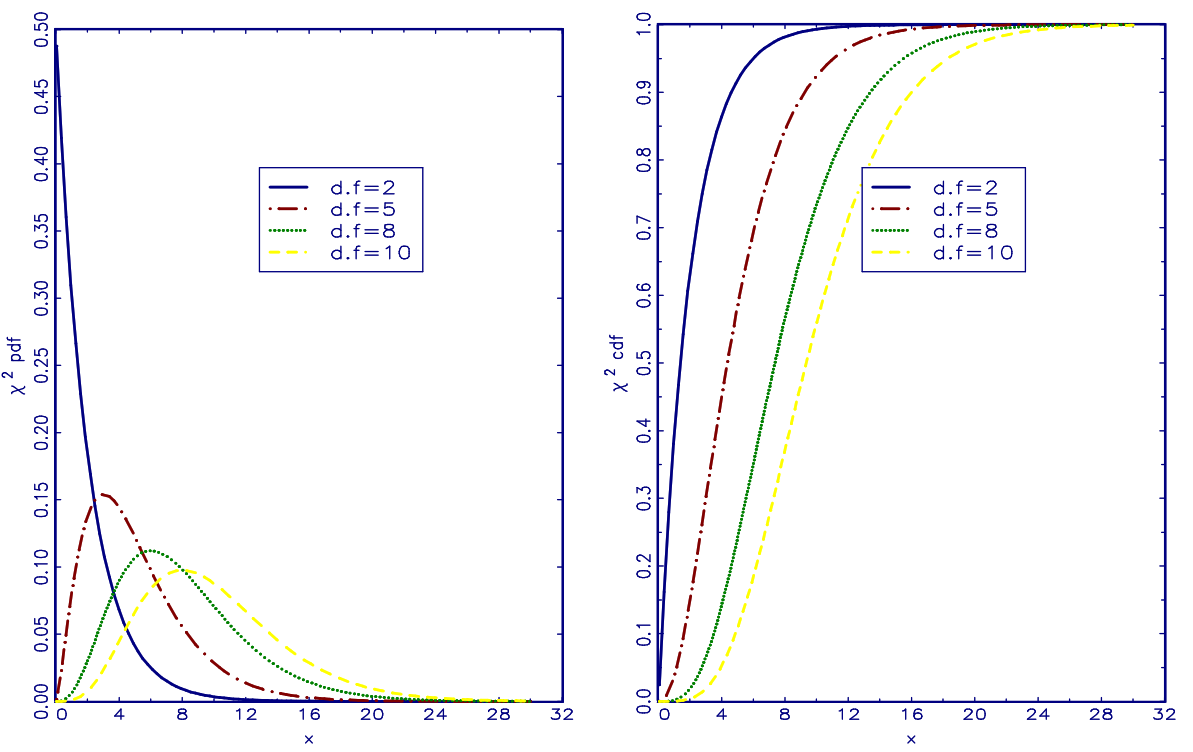
\includegraphics[scale=.22]{figuras/dist2.png}
		\end{figure}
	los gráficos de esta distribución son denotadas como $\chi^{2}(g.l.)$ o $\chi_{(g.l.)}^{2}$
\end{frame}
%------------------------------------------------
\begin{frame}{Distribución t-student}
	El siguiente panel de gráficos muestra la fdp y la fda de una t-student bajo diferentes grados de libertad.
		\begin{figure}
			\centering
			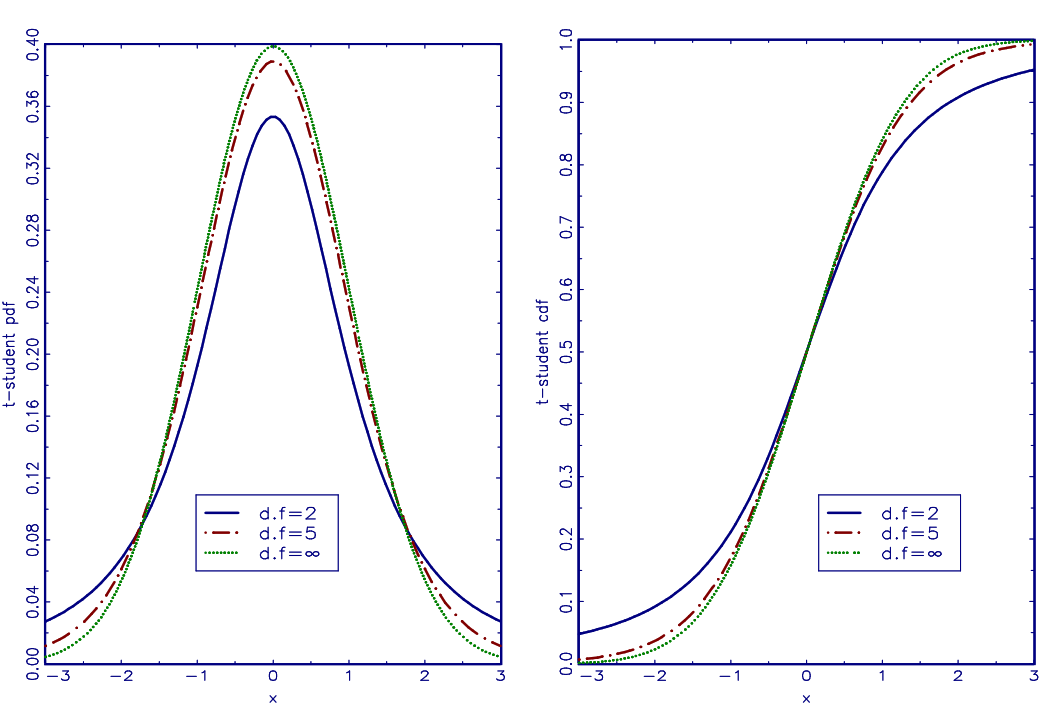
\includegraphics[scale=.22]{figuras/dist3.png}
		\end{figure}
	los gráficos de esta distribución son denotadas como $t_{g.l.}$
\end{frame}
%------------------------------------------------
\begin{frame}{Distribución F}
	El siguiente panel de gráficos muestra la fdp y la fda de una F bajo diferentes grados de libertad.
		\begin{figure}
			\centering
			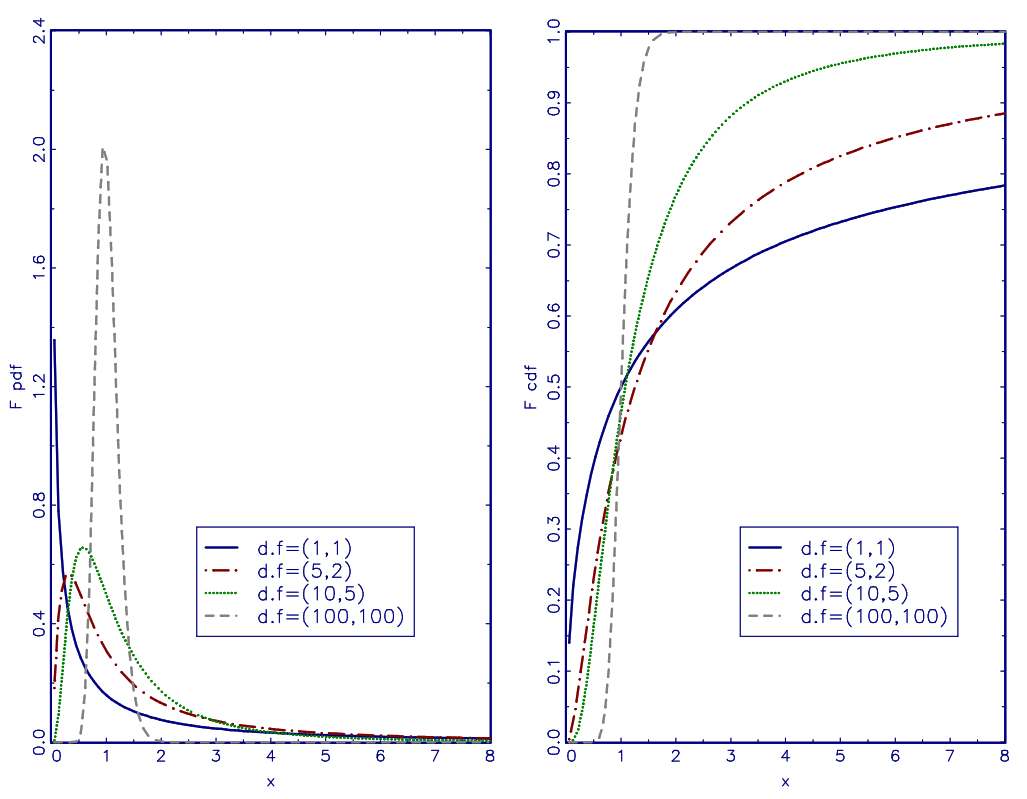
\includegraphics[scale=.22]{figuras/dist4.png}
		\end{figure}
	los gráficos de esta distribución son denotadas como $F(g.l. 1 , g.l. 2)$
\end{frame}
%------------------------------------------------
\begin{frame}{Relación entre funciones}
	\begin{figure}
		\centering
		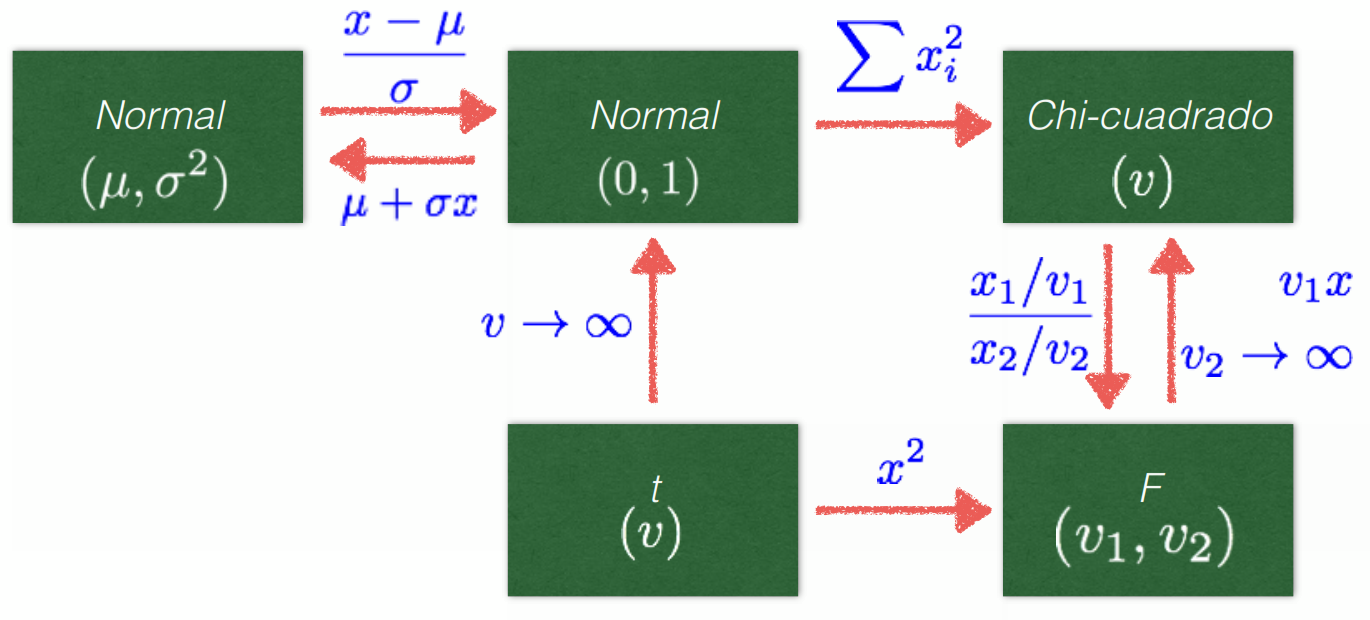
\includegraphics[scale=.30]{figuras/funciones.png}
	\end{figure}
\end{frame}
%------------------------------------------------
\begin{frame}{¿Sabes cómo leer tablas estadísticas?}
	\begin{description}
		\item[Prob 1] En la Prueba 1, los estudiantes no informaron los valores de las tablas estadísticas. Les pido que calculen los valores de $F (2, 26)$, $\chi^2(60)$ con un nivel de significancia de 0.05; y $t_{60}$ con un nivel de significancia de 0.005 (considere dos colas para eso). [\textit{Sugerencia: un nivel de significancia = área bajo la curva comenzando desde la izquierda}]
			\begin{align*}
				&\textup{Respuestas}\\
				&F(2,6)=3.37\\
				&\chi^{2}(60)=79.08\\
				&t_{60}=2.66
			\end{align*}
		\item[Prob 2] x es una variable aleatoria normal  estándar, calcule lo siguiente $a) P (x> 0)$, $b) P (x> 2.99)$ y $c) P (1.96> x> 1.96)$
	\end{description}
\end{frame}

%-----------------------------------------------------------------
\subsection{Aproximaciones de muestras grandes}
%-----------------------------------------------------------------
{\small
\begin{frame}{Propiedades de la Ley de Grandes Números y Consistencia}
	\begin{itemize}
		\item La ley de los grandes números (LGN) o la ley de los promedios
		\item Debido a que tenemos un límite de observaciones o una pequeña muestra observable, necesitamos aproximar las distribuciones utilizando una basada en muestras grandes (distribución asintótica).
		\item Para usar una aproximación para distribuciones (en este caso la normal) necesitamos (al menos) estar seguros de que la media se conoce en muestras grandes. Para ello nos basamos en el LGN y el teorema del límite central.
		\item La LGN dice que cuando el tamaño de la muestra es grande, el promedio muestral ($\overline{Y}$) estará más cerca a $\mu_{Y}$ con una alta probabilidad. Denotamos esta propiedad como $\overline{Y} \xrightarrow{p} \mu_{Y}$.
		\item Formalmente, si $Y$ son independiente e idénticamente distribuidas con $E(Y)=\mu_{Y}$ y si los valores atípicos son poco probables, entonces $\overline{Y} \xrightarrow{p} \mu_{Y}$.
	\end{itemize}
\end{frame}
}
%------------------------------------------------
\begin{frame}{Propiedades de la Ley de Grandes Números y Consistencia}
	En el caso de que $X \thicksim \chi^{2}(2)$; sabemos que $E[\chi^{2}(2)]=\mu_{\chi^{2}}=2$ y var$[\chi^{2}(2)]$ = 4 $< \infty$. Por lo tanto tenemos que $\overline{X} \xrightarrow{p} \mu_{X}$.
		\begin{figure}
			\centering
			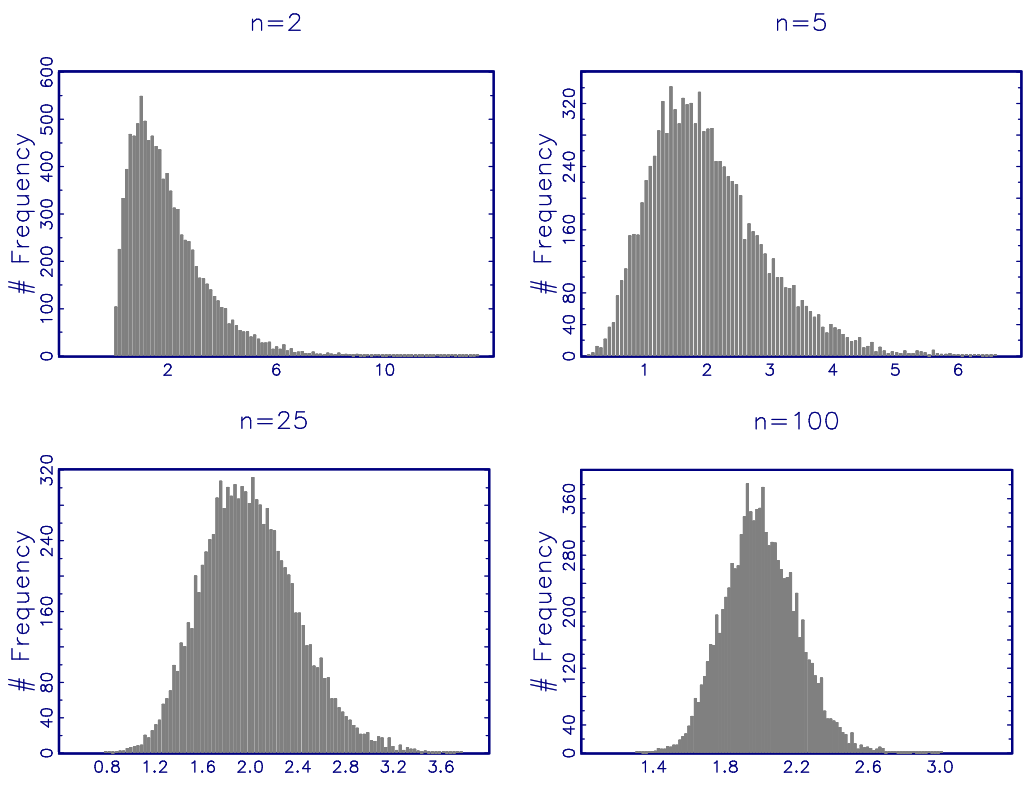
\includegraphics[scale=.22]{figuras/lgn.png}
		\end{figure}
\end{frame}
%------------------------------------------------
\begin{frame}{Teorema del Límite Central}
	\begin{itemize}
		\item Ahora, sabemos que esta nueva variable $\overline{Y}$ tiene una media igual a $\mu_{Y}$ en muestras grandes. ¿Cuál es la forma de la distribución límite (o asintótica)?
		\item El teorema del límite central (CLT) dice que la distribución de una media muestral ($\overline{Y}$) está bien aproximada por una distribución normal cuando $n$ es grande.
		\item Recuerde que la media es $\mu_{Y}$ y la varianza $\frac{\sigma_{Y}^{2}}{n}$ para $Y$.
		\item La distribución asintótica de $\overline{Y}$ no depende de la distribución de $Y$.
		\item Esta simplificación (a punto de utilizar distribuciones normales como asintóticas) subyace a la teoría de la regresión.
	\end{itemize}
\end{frame}
%------------------------------------------------
\begin{frame}{Teorema del Límite Central}
	En el caso de $X \thicksim U(0,1)$; sabemos que $E[X]=0.5$ y var$[X]=\frac{1}{12}$. Por el TLC $\overline{X} \xrightarrow{d} N(0.5, \sigma_{\overline{X}}^{2})$.
		\begin{figure}
			\centering
			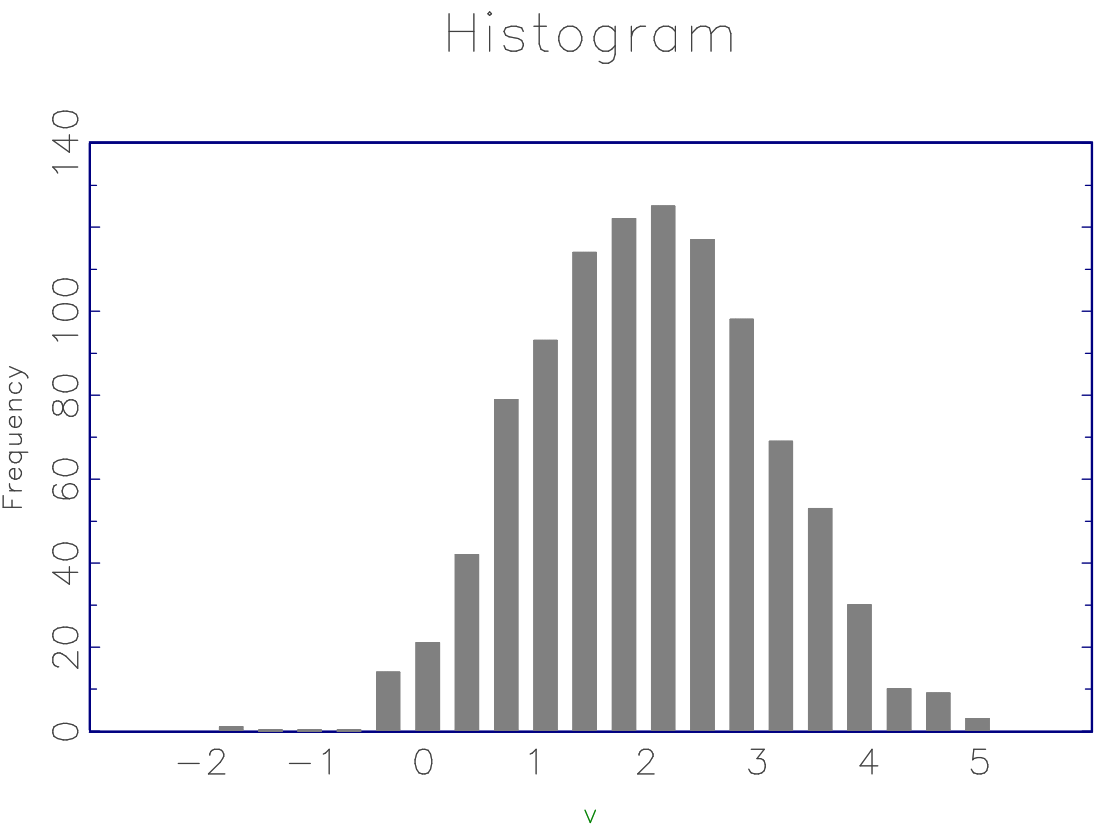
\includegraphics[scale=.22]{figuras/tlc.png}
		\end{figure}
\end{frame}

%-----------------------------------------------------------------
\subsection{Conclusiones}
%-----------------------------------------------------------------
\begin{frame}{Conclusiones}
	\begin{itemize}
		\item Recuerde que el valor esperado, cuando existe, es casi con seguridad el límite de la media muestral a medida que el tamaño de la muestra crece hasta el infinito. Por tanto, el valor esperado puede entenderse por la ley de los grandes números
		\item La expectativa es un operador lineal.
		\item La independencia no implica correlación, pero lo contrario no es válido.
		\item La media, la desviación estándar, la asimetría y la curtosis son momentos de las distribuciones.
		\item LLN dice que cuando el tamaño de la muestra es grande, la media de la muestra $(\overline{Y})$ estará cerca de $\mu_{Y}$ con una probabilidad muy alta
		\item La distribución asintótica de $\overline{Y}$ no depende de la distribución de $Y$.
	\end{itemize}
\end{frame}